\chapter{Numerical applications}\label{ch:applications}

\epigraph{The most obvious characteristic of science is its application: the fact that, as a consequence of science, one has a power to do things. And the effect this power has had need hardly be mentioned. The whole industrial revolution would almost have been impossible without the development of science.}{\textit{Richard Feynman \\ The Meaning of It All: Thoughts of a Citizen-Scientist}}
\minitoc

\lettrine{\color{theme}{T}}he proposed finite element discretization can be employed for different numerical applications. The chapter is organized as follows:
\begin{itemize}
	\item a boundary stabilization problem for the Kirchhoff plate and for the irrotational shallow water equations is presented in \secref{sec:bd_stab};
	\item Sec. \ref{sec:mixbd_enfor} presents a comparison of the Lagrange multiplier \ref{sec:lagrMul} and the virtual domain decomposition method \ref{sec:vdd} for the enforcement of mixed boundary conditions;
	\item a thermoelastic problem for which an analytic solution is available is illustrated in \secref{sec:thelas_wave}.
\end{itemize}



\section{Boundary stabilization}\label{sec:bd_stab}

In this section, we consider the boundary stabilization of a cantilever Kirchhoff plate of the irrotational shallow water equations. For pHs a simple proportional gain assures asymptotic system of the system thanks to the LaSalle’ invariance principle \cite[Proposition 6.2]{duindam2009}. This can be used to achieve stabilization of the undeformed configuration of the Kirchhoff plate. For the shallow water equations a reference is also added to stabilizes the system around a certain fluid height.


\subsection{Cantilever Kirchhoff plate}\label{sec:bd_stabKP}

\begin{figure}[t]
	\centering
	\includegraphics[width=0.5\textwidth]{part_3/applications/bs_Kirchh/plate_controlled.eps}
	\caption{Cantilever plate subjected to a control forces on the lateral sides.}
	\label{fig:plate_controlled}
\end{figure}

Consider the problem (illustrated in Fig. \ref{fig:plate_controlled})
\begin{equation*}\small
\begin{bmatrix}
\rho h & 0 \\ 
\bm{0} & \bm{\mathcal{C}_b} \\
\end{bmatrix}
\diffp{}{t}
\begin{pmatrix}
e_w \\ \bm{E}_\kappa \\
\end{pmatrix} = 
\begin{bmatrix}
0 & -\div\Div \\ 
\Hess & \bm{0} \\
\end{bmatrix}
\begin{pmatrix}
e_w \\ \bm{E}_\kappa \\
\end{pmatrix} \qquad (x, y) \in \Omega = [0, 1]\times[0,1]
\end{equation*}
subjected to the following Dirichlet homogeneous conditions
\begin{align*}
\begin{aligned}
\partial_t e_w|_{\Gamma_D} &= 0, \\
\partial_x e_w|_{\Gamma_D} &= 0, \\
\end{aligned} \qquad {\Gamma_D} &= \left\{x = 0 \right\},
\end{align*}
and Neumann boundary control
\begin{align*}
\begin{aligned}
u_{\partial, q} & = \widetilde{q}_n|_{\Gamma_N} = -\bm{n} \cdot \Div \bm{E}_\kappa - \partial_{\bm{s}} (\bm{E}_\kappa \cddot (\bm{n} \otimes \bm{s}))|_{\Gamma_N},\\
u_{\partial, m} &= m_{nn}|_{\Gamma_N} =\bm{E}_\kappa \cddot (\bm{n}\otimes \bm{n})|_{\Gamma_N}, \; \\
\end{aligned} \qquad {\Gamma_N} &= \left\{y = 0 \cup x=1 \cup y=1 \right\}.
\end{align*}
The corresponding boundary outputs read
\begin{equation*}
\begin{aligned}
y_{\partial, q} &= e_w|_{\Gamma_N}, \\
y_{\partial, m} &=\partial_{\bm{n}} e_w|_{\Gamma_N}.
\end{aligned}
\end{equation*}
The initial conditions (compatible with the constraints) are given by
\[
e_w(x,y,0) = x^2 y (y-1), \qquad \bm{E}_\kappa(x,y,0) ={0}.
\]
The following control law asymptotically stabilizes the system (cf. \cite{lagnese1989})
\begin{equation}\label{eq:ctrllaw_Kir}
\begin{aligned}
u_{\partial, q} &= - k_q e_w|_{\Gamma_N} = - k_q y_{\partial, q}, \\
u_{\partial, m} &= - k_m \partial_{\bm{n}} e_w|_{\Gamma_N}  = - k_m y_{\partial, m}, \\
\end{aligned} \qquad
\begin{aligned}
 k_q&>0, \\
 k_m&>0.
\end{aligned}
\end{equation}
\\

The discretization is performed as in \eqref{eq:pHsys_findim_kirchh_hess}. Variables $e_w$ and $\bm{E}_\kappa$ are discretized using the Argyris element and Discontinuous Galerkin elements of order 3. A structured mesh with 6 elements for side is used. The Dirichlet conditions are imposed weakly using Lagrange multipliers (cf. \eqref{eq:pHsys_infdim_mult1} and Remark \ref{rmk:BellArg}), that are discretized using Lagrange polynomials of order 2. The resulting system read

\begin{equation}\label{eq:pHsys_findim_bdKir_open}
\begin{aligned}
\begin{bmatrix}
\mathbf{M}_{\rho h} & \mathbf{0} & \mathbf{0}\\
\mathbf{0} & \mathbf{M}_{\bm{\mathcal{C}}_b} & \mathbf{0}\\
\mathbf{0} & \mathbf{0} & \mathbf{0}\\
\end{bmatrix}
\begin{pmatrix}
\dot{\mathbf{e}}_{w} \\
\dot{\mathbf{e}}_{\kappa} \\
\dot{\bm{\lambda}}_{\Gamma_D} \\
\end{pmatrix}
&= \begin{bmatrix}
\mathbf{0} & - \mathbf{D}_{\Hess}^\top & \mathbf{B}_{\Gamma_D}\\
\mathbf{D}_{\Hess} & \mathbf{0} & \mathbf{0} \\
-\mathbf{B}_{\Gamma_D}^\top & \mathbf{0} & \mathbf{0} \\
\end{bmatrix} 
\begin{pmatrix}
{\mathbf{e}}_{w} \\
{\mathbf{e}}_{\kappa} \\
{\bm{\lambda}}_{\Gamma_D} \\
\end{pmatrix} + 
\begin{bmatrix}
\mathbf{B}_{w, \Gamma_N} & \mathbf{B}_{\partial_{\bm{n}} w, \Gamma_N}\\
\mathbf{0} & \mathbf{0} \\
\mathbf{0} & \mathbf{0} \\
\end{bmatrix}
\begin{bmatrix}
\mathbf{u}_{\partial, q} \\
\mathbf{u}_{\partial, m} \\
\end{bmatrix}, \\
\begin{bmatrix}
\mathbf{M}_{\Gamma_N} & \mathbf{0} \\
\mathbf{0} & \mathbf{M}_{\Gamma_N} \\
\end{bmatrix}
\begin{pmatrix}
\mathbf{y}_{\partial, q} \\
\mathbf{y}_{\partial, m} \\
\end{pmatrix}
&= \begin{bmatrix}
\mathbf{B}_{w, \Gamma_N}^\top & \mathbf{0} &  \mathbf{0} \\
\mathbf{B}_{\partial_{\bm{n}} w, \Gamma_N}^\top & \mathbf{0} & \mathbf{0} \\
\end{bmatrix}
\begin{pmatrix}
{\mathbf{e}}_{w} \\
{\mathbf{e}}_{\kappa} \\
{\bm{\lambda}}_{\Gamma_D} \\
\end{pmatrix},
\end{aligned}
\end{equation}
where $\mathbf{B}_{\Gamma_D} = [\mathbf{B}_{w, \Gamma_D} \; \mathbf{B}_{\partial_n w, \Gamma_D}]$. The discretization of the control law \eqref{eq:ctrllaw_Kir} provides
\begin{equation}
\begin{aligned}
\mathbf{u}_{\partial, q} &= -k_q \mathbf{y}_{\partial, q} = - k_q \mathbf{M}_{\Gamma_N}^{-1} \mathbf{B}_{w, \Gamma_N}^\top \mathbf{e}_w, \\
\mathbf{u}_{\partial, m} &= -k_m \mathbf{y}_{\partial, m} = - k_m \mathbf{M}_{\Gamma_N}^{-1} \mathbf{B}_{\partial_{\bm{n}} w, \Gamma_N}^\top \mathbf{e}_w.
\end{aligned}
\end{equation}
System \eqref{eq:pHsys_findim_bdKir_open} now reads
\begin{equation}
\begin{bmatrix}
\mathbf{M}_{\rho h} & \mathbf{0} & \mathbf{0}\\
\mathbf{0} & \mathbf{M}_{\bm{\mathcal{C}}_b} & \mathbf{0}\\
\mathbf{0} & \mathbf{0} & \mathbf{0}\\
\end{bmatrix}
\begin{pmatrix}
\dot{\mathbf{e}}_{w} \\
\dot{\mathbf{e}}_{\kappa} \\
\dot{\bm{\lambda}}_{\Gamma_D} \\
\end{pmatrix}
= \begin{bmatrix}
-\mathbf{R}_w  & - \mathbf{D}_{\Hess}^\top & \mathbf{B}_{\Gamma_D}\\
\mathbf{D}_{\Hess} & \mathbf{0} & \mathbf{0} \\
-\mathbf{B}_{\Gamma_D}^\top & \mathbf{0} & \mathbf{0} \\
\end{bmatrix} 
\begin{pmatrix}
{\mathbf{e}}_{w} \\
{\mathbf{e}}_{\kappa} \\
{\bm{\lambda}}_{\Gamma_D} \\
\end{pmatrix}.
\end{equation}
The matrix 
$$\mathbf{R}_w = k_q \mathbf{B}_{w, \Gamma_N} \mathbf{M}_{\Gamma_N}^{-1} \mathbf{B}_{w, \Gamma_N}^\top + k_m \mathbf{B}_{\partial_{\bm{n}} w, \Gamma_N} \mathbf{M}_{\Gamma_N,}^{-1} \mathbf{B}_{\partial_{\bm{n}} w, \Gamma_N}^\top \succ 0$$
 is positive definitive because of the collocated input-output feature of pH systems. The energy rate evaluates to \cite[Theorem 13]{beattie2018linear}
\[\dot{H} _{d} = - \mathbf{e}_{w}^\top \; \mathbf{R}_w \; \mathbf{e}_{w} \le 0. \]
Therefore, the Hamiltonian energy is a Lyapunov function and the asymptotic stability of configuration $\mathbf{e}_{w} = \mathbf{0}, \; \mathbf{e}_{\kappa} = \mathbf{0}$ is deduced using LaSalle' invariance  principle. \\


\begin{table}[t]
	\centering
	\begin{tabular}{|c|c|}
		\hline 
		\multicolumn{2}{|c|}{Plate Parameters} \\ 
		\hline 
		$E$ & $70\; \mathrm{[GPa]}$ \\ 
		$\rho$ & $2700\; \mathrm{[kg \cdot m^3]}$ \\ 
		$\nu$& 0.35 \\ 
		$h/L$& 0.05 \\ 
		$L_x = L_y$& $1\; \mathrm{[m]}$\\ 
		\hline 
	\end{tabular} \hspace{1cm}
	\begin{tabular}{|c|c|}
		\hline 
		\multicolumn{2}{|c|}{Simulation Settings} \\
		\hline 
		Integrator & St\"ormer-Verlet \\
		$\Delta t $ & $1 \; \mathrm{[\mu s]}$ \\  
		N$^\circ$ FE & 6 \\
		FE spaces & Argyris $\times$ DG$_3$ $\times$ CG$_2$\\
		$t_{\text{end}}$ & $5\; \mathrm{[s]}$\\ 
		\hline 
	\end{tabular} 
	\captionsetup{width=0.95\linewidth}
	\vspace{1mm}
	\captionof{table}{Settings and parameters for the boundary control of the Kirchhoff plate.}
	\label{tab:parKir_damp}
\end{table}

The parameters for the numerical simulation are given in Table~\ref{tab:parKir_damp}. The controller gains are set to 
\begin{equation}
	k_q = 10, \qquad k_m = 10.
\end{equation}

The system is simulated using a St\"ormer-Verlet time integrator \cite{hairer2003geometric} using a time step $\Delta t = 10^{-6}$ for a total simulation time of $t_{\text{end}} = 5 \; \mathrm{[s]}$. The Lagrange multiplier is eliminated using a projection method \cite{benner2015time}. The control law is activated after 1 second. Snapshots of the simulation are reported in Fig. \ref{fig:SnapDamp_Kir}. The discrete Hamiltonian goes almost to zero in 4 seconds (Fig. \ref{fig:H_bs_Kirchhoff}).


\begin{figure}[htb]
	\centering
	\includegraphics[width=0.48\linewidth]{part_3/applications/bs_Kirchh/Hamiltonian.eps}
	\caption{Hamiltonian trend for the cantilever Kirchhoff plate.}
	\label{fig:H_bs_Kirchhoff}
\end{figure}

\begin{figure*}[p]
	\centering
	\subfloat[$t=0.15 \; \mathrm{[s]}$]{\includegraphics[height=0.2\textheight]{part_3/applications/bs_Kirchh/Snapshot_t30.eps}%
		\label{fig:Damp_1_Kir}}
	\subfloat[$t=0.30 \; \mathrm{[s]}$]{\includegraphics[height=0.2\textheight]{part_3/applications/bs_Kirchh/Snapshot_t60.eps}%
		\label{fig:Damp_2_Kir}}
	\hfil
	\subfloat[$t=1.40 \; \mathrm{[s]}$]{\includegraphics[height=0.2\textheight]{part_3/applications/bs_Kirchh/Snapshot_t280.eps}%
		\label{fig:Damp_3_Kir}}
	\subfloat[$t=1.60 \; \mathrm{[s]}$]{\includegraphics[height=0.2\textheight]{part_3/applications/bs_Kirchh/Snapshot_t320.eps}%
		\label{fig:Damp_4_Kir}}
	\hfil
	\subfloat[$t=2.40 \; \mathrm{[s]}$]{\includegraphics[height=0.2\textheight]{part_3/applications/bs_Kirchh/Snapshot_t480.eps}%
		\label{fig:Damp_5_Kir}}
	\subfloat[$t=2.85 \; \mathrm{[s]}$]{\includegraphics[height=0.2\textheight]{part_3/applications/bs_Kirchh/Snapshot_t570.eps}%
		\label{fig:Damp_6_Kir}}
	\hfil
	\subfloat[$t=3.65 \; \mathrm{[s]}$]{\includegraphics[height=0.2\textheight]{part_3/applications/bs_Kirchh/Snapshot_t730.eps}%
		\label{fig:Damp_7_Kir}}
	\subfloat[$t=5 \; \mathrm{[s]}$]{\includegraphics[height=0.2\textheight]{part_3/applications/bs_Kirchh/Snapshot_t1000.eps}%
		\label{fig:Damp_8_Kir}}
	\hfil
	\caption{Snapshots at different times of the simulation of the boundary controlled cantilever Kirchhoff plate.}
	\label{fig:SnapDamp_Kir}
	\hfil
\end{figure*}



\subsection{Irrotational shallow water equations}
In this section we consider the boundary stabilization of a circular water tank via proportional feedback. We recall the system of equations \eqref{eq:pHsys_shwater}

\begin{equation}
\begin{aligned}
\diffp{}{t}
\begin{pmatrix}
\alpha_h \\
\bm{\alpha}_v \\
\end{pmatrix} &= 
\begin{bmatrix}
0 & -\div \\
-\grad & \bm{0}
\end{bmatrix}
\begin{pmatrix}
e_h\\
\bm{e}_v\\
\end{pmatrix}, \qquad (x,y) \in \Omega = \{x^2 + y^2 \le R \}, \\
\begin{pmatrix}
e_h\\
\bm{e}_v\\
\end{pmatrix} &= \begin{pmatrix}
\delta_{\alpha_h} H\\
\delta_{\bm{\alpha}_v} H\\
\end{pmatrix}
\end{aligned}
\end{equation}
with 
\begin{equation}
H(\alpha_h, \bm{\alpha}_v) = \energy{\frac{1}{\rho} \alpha_h \norm{\bm{\alpha}_v}^2 + \rho g \alpha_h^2},
\end{equation}
under Neumann boundary control 
\begin{equation}
	{u}_\partial = - \bm{e}_v \cdot \bm{n}\vert_{\partial\Omega} = - \frac{1}{\rho}\alpha_h \bm{\alpha}_v \cdot\bm{n}\vert_{\partial\Omega}. 
\end{equation}
The corresponding output reads
\begin{equation}
{y}_\partial = {e}_h\vert_{\partial\Omega} = (\rho g \alpha_h + \frac{1}{2\rho} \norm{\bm{\alpha}_v}^2)\vert_{\partial\Omega}.
\end{equation}

 The initial conditions are
\begin{equation}
\begin{aligned}
\alpha_h(x, y, 0) &= h^{\text{des}} + 10^{-1} \sin(\pi r/R) \cos(2 \theta), \qquad r = \sqrt{x^2 + y^2}, \qquad \theta = \arctan(y/r), \\
\bm\alpha_v(x, y, 0) &= \bm{0},
\end{aligned}
\end{equation}
where $ h^{\text{des}}$ is the desired fluid height. It is known that a proportional controller exponentially stabilizes the system \cite{dos2008boundary}. Here, we use a simple control for stabilizing the system around the desired point $h^*$
\begin{equation}\label{eq:ctrllaw_SWE}
u_\partial = -k (y_\partial - y_\partial^{\text{des}}), \qquad y_\partial^{\text{des}}= \rho g h^{\text{des}}, \quad k>0.
\end{equation}
This control law ensures that the Lyapunov functional
\begin{equation}
	V = \frac{1}{2} \int_{\Omega}\left\{\frac{1}{2} \rho g (\alpha_h - \alpha_h^{\text{des}})^2 + \frac{1}{2\rho} \alpha_h \norm{\bm{\alpha}_v}^2 \right\} d\Omega \ge 0,
\end{equation}
where $\alpha_h^{\text{des}}=h^{\text{des}}$, has negative semi definite time derivative
\begin{equation}
	\dot{V} = -k \int_{\partial \Omega}\left({y}_\partial - {y}_\partial^{\text{des}} \right)^2 \d{\Gamma} \le 0.
\end{equation}
By the LaSalle' principle \cite{henry2006geometric} the point 
\begin{equation}
	\alpha_h = h^{\text{des}}, \qquad \bm{\alpha}_v = \bm{0},
\end{equation}
is asymptotically stable. \\

The discretization is performed as in \eqref{eq:pHsys_findim_shwater}. Variable $\alpha_h$ is discretized suing Lagrange polynomials of order 1. Discontinuous Galerkin of order 0 defined on the domain and on the boundary are used for $\bm{\alpha}_v, \bm{u}_\partial$.
\begin{equation}\label{eq:pHsys_findim_shwater_ctrl}
\begin{aligned}
\begin{pmatrix}
\dot{\bm{\alpha}}_{d, h} \\
\dot{\bm{\alpha}}_{d, v} \\
\end{pmatrix}
&= \begin{bmatrix}
\mathbf{0} &  \mathbf{M}_h^{-1} \mathbf{D}_{\grad}^\top \mathbf{M}_v^{-1} \\
-\mathbf{M}_v^{-1} \mathbf{D}_{\grad} \mathbf{M}_h^{-1} & \mathbf{0} \\
\end{bmatrix} 
\begin{pmatrix}
\partial_{\bm{\alpha}_{d, h}} H_d(\bm{\alpha}_{d, h},\; \bm{\alpha}_{d, v})\\
\partial_{\bm{\alpha}_{d, v}} H_d(\bm{\alpha}_{d, h},\; \bm{\alpha}_{d, v})\\
\end{pmatrix} + 
\begin{bmatrix}
\mathbf{B}_h \\
\mathbf{0}\\
\end{bmatrix}
\mathbf{u}_\partial, \\
\mathbf{M}_\partial {\mathbf{y}_\partial} &= \begin{bmatrix}
\mathbf{B}_h^\top & \mathbf{0}
\end{bmatrix}\begin{pmatrix}
\partial_{\bm{\alpha}_{d, h}} H_d(\bm{\alpha}_{d, h},\; \bm{\alpha}_{d, v})\\
\partial_{\bm{\alpha}_{d, v}} H_d(\bm{\alpha}_{d, h},\; \bm{\alpha}_{d, v})\\
\end{pmatrix}.
\end{aligned}
\end{equation}
The control law \eqref{eq:ctrllaw_SWE}, once discretized, is expressed as
\begin{equation}
	\mathbf{u}_\partial = -k (\mathbf{y}_\partial - \mathbf{y}_\partial^{\text{des}}),
\end{equation}
where $\mathbf{y}_\partial^{\text{des}} = \mathbf{M}_\partial^{-1}\int_{\partial\Omega} \rho g h^{\text{des}} \phi_\partial(s) \d\Gamma$. The closed loop system is then
\begin{equation}\label{eq:pHsys_findim_shwater_ctrlcl}
\begin{pmatrix}
\dot{\bm{\alpha}}_{d, h} \\
\dot{\bm{\alpha}}_{d, v} \\
\end{pmatrix}
= \begin{bmatrix}
-\mathbf{R}_h &  \mathbf{M}_h^{-1} \mathbf{D}_{\grad}^\top \mathbf{M}_v^{-1} \\
-\mathbf{M}_v^{-1} \mathbf{D}_{\grad} \mathbf{M}_h^{-1} & \mathbf{0} \\
\end{bmatrix} 
\begin{bmatrix}
\partial_{\bm{\alpha}_{d, h}} H_d(\bm{\alpha}_{d, h},\; \bm{\alpha}_{d, v})\\
\partial_{\bm{\alpha}_{d, v}} H_d(\bm{\alpha}_{d, h},\; \bm{\alpha}_{d, v})\\
\end{bmatrix} + 
\begin{bmatrix}
\mathbf{B}_h \\
\mathbf{0}\\
\end{bmatrix}
k \mathbf{y}_\partial^{\text{des}}, 
\end{equation}
Again the matrix 
\begin{equation*}
	\mathbf{R}_h = k \mathbf{B}_h \mathbf{M}_\partial^{-1} \mathbf{B}_h^\top \succ 0
\end{equation*}
is positive definite and the discretized Lyapunov function rate reads
\begin{equation*}
\dot{V}_d = - \partial_{\bm{\alpha}_{d, h}} H_d(\bm{\alpha}_{d, h},\; \bm{\alpha}_{d, v})^\top \mathbf{R}_h \partial_{\bm{\alpha}_{d, h}} H_d(\bm{\alpha}_{d, h},\; \bm{\alpha}_{d, v}) \le 0.
\end{equation*}

\begin{table}[th]
	\centering
	\begin{tabular}{|c|c|}
		\hline 
		\multicolumn{2}{|c|}{Parameters} \\ 
		\hline 
		$\rho$ & $1000\; \mathrm{[kg \cdot m^3]}$ \\ 
		$g$& $10\; \mathrm{[m/s^2]}$ \\ 
		$R$& $1\; \mathrm{[m]}$\\ 
		$h^{\text{des}}$& $1\; \mathrm{[m]}$ \\ 
		\hline 
	\end{tabular} \hspace{1cm}
	\begin{tabular}{|c|c|}
		\hline 
		\multicolumn{2}{|c|}{Simulation Settings} \\
		\hline 
		Integrator & Runge-Kutta 45 \\
		N$^\circ$ FE along $R$ & 20 \\
		FE spaces & CG$_1$ $\times$ DG$_0$ $\times$ DG$_0$\\
		$t_{\text{end}}$ & $3\; \mathrm{[s]}$\\ 
		\hline 
	\end{tabular} 
	\captionsetup{width=0.95\linewidth}
	\vspace{1mm}
	\captionof{table}{Settings and parameters for the irrotational shallow water equations.}
	\label{tab:parSWE_damp}
\end{table}

The parameters for the simulation are reported in Table. \eqref{tab:parSWE_damp}. The controller gain is set to $k = 10^{-3}$. The control law is activated after $0.5$ seconds. The system is simulated using a Runge-Kutta method. Snapshots are collected in Fig. \ref{fig:SnapDamp_SWE}. The discretized Hamiltonian and Lyapunov functional trends (Fig. \ref{fig:HL_SWE}) clearly show that, while the Lyapunov function monotonically decrease, the Hamiltonian oscillates around the desired equilibrium.



\begin{figure}[htb]%
	\centering
	\subfloat[][Totat energy (Hamiltonian)]{%
		\label{fig:H_SWE}%
		\includegraphics[width=0.48\columnwidth]{part_3/applications/bs_SWE/Hamiltonian.eps}}%
	\hspace{8pt}%
	\subfloat[][Lyapunov function]{%
		\label{fig:L_SWE}%
		\includegraphics[width=0.48\columnwidth]{part_3/applications/bs_SWE/Lyapunov.eps}} \\
	\caption{Total energy and Lyapunov function for the shallow water equations.}%
	\label{fig:HL_SWE}%
\end{figure}


\begin{figure*}[p]
	\centering
	\subfloat[$t=0 \; \mathrm{[s]}$]{\includegraphics[height=0.2\textheight]{part_3/applications/bs_SWE/Snap_n1.eps}%
		\label{fig:Damp_1_SWE}}
	\subfloat[$t=0.42 \; \mathrm{[s]}$]{\includegraphics[height=0.2\textheight]{part_3/applications/bs_SWE/Snap_n43.eps}%
		\label{fig:Damp_2_SWE}}
	\hfil
	\subfloat[$t=0.85 \; \mathrm{[s]}$]{\includegraphics[height=0.2\textheight]{part_3/applications/bs_SWE/Snap_n86.eps}%
		\label{fig:Damp_3_SWE}}
	\subfloat[$t=1.28 \; \mathrm{[s]}$]{\includegraphics[height=0.2\textheight]{part_3/applications/bs_SWE/Snap_n129.eps}%
		\label{fig:Damp_4_SWE}}
	\hfil
	\subfloat[$t=1.71 \; \mathrm{[s]}$]{\includegraphics[height=0.2\textheight]{part_3/applications/bs_SWE/Snap_n171.eps}%
		\label{fig:Damp_5_SWE}}
	\subfloat[$t=2.14 \; \mathrm{[s]}$]{\includegraphics[height=0.2\textheight]{part_3/applications/bs_SWE/Snap_n214.eps}%
		\label{fig:Damp_6_SWE}}
	\hfil
	\subfloat[$t=2.57 \; \mathrm{[s]}$]{\includegraphics[height=0.2\textheight]{part_3/applications/bs_SWE/Snap_n257.eps}%
		\label{fig:Damp_7_SWE}}
	\subfloat[$t=3 \; \mathrm{[s]}$]{\includegraphics[height=0.2\textheight]{part_3/applications/bs_SWE/Snap_n300.eps}%
		\label{fig:Damp_8_SWE}}
	\hfil
	\caption{Snapshots at different times of the simulation for the boundary controlled irrotational shallow water equations.}
	\label{fig:SnapDamp_SWE}
	\hfil
\end{figure*}


\section{Mixed boundary conditions enforcement}\label{sec:mixbd_enfor}
In this section the Lagrange multiplier method \secref{sec:lagrMul} and the virtual domain decomposition method \secref{sec:vdd} are compared for two problems:
\begin{enumerate}
	\item a reference tracking problem for the Euler-Bernoulli beam;
	\item a vibroacoustic application.
\end{enumerate}

\subsection{Motion planning of a thin beam}
Consider the motion planning problem for the Euler Bernoulli beam \cite[Chapter 12]{krstic2008boundary}
\begin{align}
\partial_{tt} w + \partial_{xxxx} w = 0,  \qquad x\in \Omega=\{0, 1\} \label{eq:classEB_1}\\
\partial_{xx} w(0, t) = 0, \qquad \partial_{xxx} w (0, t) = 0, \label{eq:bcEB_hom}\\
w^r(0, t) = \sin(\omega t), \qquad \partial_x w^r(0, t) = 0. \label{eq:bcEB_r}
\end{align}
The equation \eqref{eq:classEB_1} represents the Euler-Bernoulli beam \eqref{eq:classEB} with unitary coefficients. Conditions \eqref{eq:bcEB_hom} represent an homogeneous free boundary conditions at the left side. The objective is to find controls $u_1 = w^r(1, t), \; u_2 =\partial_x w^r(1, t)$ to match the reference outputs $y_1^r = w^r(0, t), \; y_2^r=\partial_x w^r(0, t)$. The reference solution for this problem can be found by postulating the existence of a function of the form
\begin{equation*}
	w^r(x, t) = \sum_{k=0}^{\infty} a_k(t) \frac{x^k}{k !}.
\end{equation*}
Given the reference output $w^r(1, t)= \sin(\omega t)$, the reference solution assumes the form (cf. \cite[Chapter 12]{krstic2008boundary} for details)
\begin{equation}\label{eq:refsol_EB}
w^r(x, t) = \sum_{k=0}^{\infty} \omega^{2k} \frac{x^{4k}}{(4k)!}\sin(\omega t) = \frac{1}{2}[\cosh(\sqrt{\omega} x) + \cos(\sqrt{\omega} x)]\sin(\omega t).
\end{equation}
The inputs that ensure the tracking of the outputs can be computed
\begin{equation}
\begin{aligned}
w^r(1, t) = \frac{1}{2}[\cosh(\sqrt{\omega}) + \cos(\sqrt{\omega})]\sin(\omega t), \\
\partial_x w^r(1, t) = \frac{1}{2}[\sinh(\sqrt{\omega}) - \sin(\sqrt{\omega})]\sin(\omega t). \\
\end{aligned}
\end{equation}

\begin{figure}[t]%
	\centering
	\includegraphics[width=0.8\columnwidth]{part_3/applications/mixed_bd_EB/prob_definition.eps} \\
	\caption{Boundary conditions for the motion planning problem.}
	\label{fig:prob_def_EB}
\end{figure}

This problem can be equivalently cast as a boundary control pH system with mixed boundary conditions (see Fig. \ref{fig:prob_def_EB})
\begin{subequations}
	\begin{align}
	\diffp{}{t}\begin{pmatrix}
	e_w \\ e_\kappa \\
	\end{pmatrix} &= \begin{bmatrix}
	0 & -\partial_{xx} \\
	\partial_{xx} & 0 \\
	\end{bmatrix} \begin{pmatrix}
	e_w \\ e_\kappa \\
	\end{pmatrix}  \\
	\begin{pmatrix}
	u_N^1 \\
	u_N^2 \\
	u_D^1 \\
	u_D^2 \\
	\end{pmatrix} &= \begin{pmatrix}
	e_\kappa(0, t) \\
	-\partial_x e_\kappa(0, t) \\
	e_w(1, t) \\
	\partial_x e_w(1,t) \\
	\end{pmatrix} = \begin{pmatrix}
	0 \\
	0 \\
	\frac{1}{2}[\cosh(\sqrt{\omega}) + \cos(\omega)]\omega \cos(\omega t) \\
	\frac{1}{2}[\sinh(\sqrt{\omega}) - \sin(\omega)]\omega \cos(\omega t) \\
	\end{pmatrix},  \\
	\begin{pmatrix}
	y_N^1 \\
	y_N^2 \\
	y_D^1 \\
	y_D^2 \\
	\end{pmatrix}  &= \begin{pmatrix}
	-\partial_x e_w(0, t) \\
	e_w(0, t) \\
	\partial_x e_\kappa(1, t) \\
	e_\kappa(1,t) \\
	\end{pmatrix}.
	\end{align}
\end{subequations}
The inputs assures that the outputs $y_{N}^1 = -\partial_x e_w(0, t), \; y_{N}^2 = e_w(0, t)$ verify the desired trajectories
$$ y_{N}^1 =  -\partial_t \partial_x w^r(0,t) = 0, \qquad y_{N}^2 = \partial_t w^r(0, t) = \omega \cos(\omega t).
$$

Next we concisely reported the discretization strategy for the imposition of mixed boundary conditions.

\paragraph{Lagrange multipliers}
If a Lagrange multipliers is used for the Neumann boundary condition the following weak form is obtained

\begin{equation}
\begin{aligned}
\inner[\Omega]{v_w}{\partial_t e_w} &= \inner[\Omega]{v_w}{-\partial_{xx} e_\kappa} , \\
\inner[\Omega]{v_\kappa}{\partial_t e_\kappa} &= \inner[\Omega]{\partial_{xx} v_\kappa}{ e_w}  + \inner[\Gamma_N]{\begin{pmatrix}
	\partial_{\bm{n}} v_\kappa \\
	v_\kappa \\
	\end{pmatrix}}{\begin{pmatrix}
	\lambda_{N}^1 \\
	\lambda_{N}^2 \\
	\end{pmatrix}} + \inner[\Gamma_D]{\begin{pmatrix}
	\partial_{\bm{n}} v_\kappa \\
	v_\kappa \\
	\end{pmatrix}}{\begin{pmatrix}
	u_{D}^1 \\
	u_{D}^2 \\
	\end{pmatrix}}.
\end{aligned}
\end{equation}

Using a Galerkin method the following system is computed.
\begin{equation}\label{eq:pHfindim_phdae_EB}
\begin{aligned}
\begin{bmatrix}
\mathbf{M}_{w} & \mathbf{0} & \mathbf{0}\\
\mathbf{0} & \mathbf{M}_{\kappa} & \mathbf{0} \\
\mathbf{0} & \mathbf{0} & \mathbf{0} \\
\end{bmatrix}
\begin{pmatrix}
\dot{\mathbf{e}}_w\\
\dot{\mathbf{e}}_\kappa\\
\dot{\bm{\lambda}}_N \\
\end{pmatrix}
&= \begin{bmatrix}
\mathbf{0} & \mathbf{D}_{-\partial_{xx}}^\top & \mathbf{0} \\
-\mathbf{D}_{-\partial_{xx}} & \mathbf{0} & \mathbf{B}_{\kappa, \Gamma_N}  \\
\mathbf{0} & -\mathbf{B}_{\kappa, \Gamma_N}^\top & \mathbf{0} \\
\end{bmatrix}
\begin{pmatrix}
{\mathbf{e}}_w\\
{\mathbf{e}}_\kappa\\
{\bm{\lambda}}_N \\
\end{pmatrix} + \begin{bmatrix}
\mathbf{0} \\
\mathbf{B}_{\kappa, \Gamma_D} \\
\mathbf{0} \\
\end{bmatrix} \mathbf{u}_D, \\
\mathbf{y}_D  &=
\begin{bmatrix}
\mathbf{0} & \mathbf{B}_{\kappa, \Gamma_D}^\top & \mathbf{0}\\ 
\end{bmatrix}
\begin{pmatrix}
{\mathbf{e}}_p\\
{\mathbf{e}}_v\\
{\bm{\lambda}}_N \\
\end{pmatrix}.
\end{aligned}
\end{equation}
The DG1Her element \eqref{eq:DG1Her} is employed for the discretization.

\begin{figure}[t]
	\begin{minipage}[b]{0.4\linewidth}
		\centering
		\includegraphics[width=0.95\columnwidth]{part_3/applications/mixed_bd_EB/dom_split.eps} \\
		\caption{Virtual decomposition of the Euler Bernoulli beam.}
		\label{fig:dom_dec_EC}
	\end{minipage}
	\hspace{0.5cm}
	\begin{minipage}[b]{0.5\linewidth}
		\centering
		\includegraphics[width=0.95\columnwidth]{part_3/applications/mixed_bd_EB/dom_int.eps}
		\caption{Interconnection for the Euler-Bernoulli beam.}
		\label{fig:dom_int_EB}
	\end{minipage}
\end{figure}


\paragraph{Virtual domain decomposition}
For the decomposition, the beam is split into halves (see Fig. \ref{fig:dom_dec_EC}).
Applying the PFEM methodology as in \ref{sec:vdd} two finite-dimensional systems are obtained. For $\Omega_N$ the system is analogous to \eqref{eq:pHfindim_Om2}, while for $\Omega_D$ to \eqref{eq:pHfindim_Om1}.

\begin{tcolorbox}[colframe=red,title=Subdomain $\Omega_N$, coltitle=white]%%
	\begin{equation}\label{eq:pHfindim_EB_OmN}
	\begin{aligned}
	\begin{bmatrix}
	\mathbf{M}_{w}^{\Omega_N} & \mathbf{0} \\
	\mathbf{0} & \mathbf{M}_{\kappa}^{\Omega_N} \\
	\end{bmatrix}
	\begin{pmatrix}
	\dot{\mathbf{e}}_{w, \Omega_N}\\
	\dot{\mathbf{e}}_{\kappa, \Omega_N}\\
	\end{pmatrix}
	&= \begin{bmatrix}
	\mathbf{0} & -\mathbf{D}_{\partial_{xx}}^{\Omega_N \top}\\
	\mathbf{D}_{\partial_{xx}}^{\Omega_N} & \mathbf{0}\\
	\end{bmatrix}
	\begin{pmatrix}
	{\mathbf{e}}_{w, \Omega_N}\\
	{\mathbf{e}}_{\kappa, \Omega_N}\\
	\end{pmatrix} + \begin{bmatrix}
	\mathbf{B}_{w, \Gamma_{\text{int}}}^{\Omega_N}\\
	\mathbf{0}\\
	\end{bmatrix}\mathbf{u}_N^{\text{int}}, \\
	\mathbf{y}_N^{\text{int}} &=
	\begin{bmatrix}
	\mathbf{B}_{w, \Gamma_{\text{int}}}^{\Omega_N \top} & \mathbf{0}\\ 
	\end{bmatrix}
	\begin{pmatrix}
	{\mathbf{e}}_{w, \Omega_N}\\
	{\mathbf{e}}_{\kappa, \Omega_N}\\
	\end{pmatrix}.
	\end{aligned}	
	\end{equation}
\end{tcolorbox}
\begin{tcolorbox}[colframe=blue,title=Subdomain $\Omega_D$,  coltitle=white]%%
	\begin{equation}\label{eq:pHfindim_EB_OmD}
	\begin{aligned}
	\begin{bmatrix}
	\mathbf{M}_{w}^{\Omega_D} & \mathbf{0}\\
	\mathbf{0} & \mathbf{M}_{\kappa}^{\Omega_D}\\
	\end{bmatrix}
	\begin{pmatrix}
	\dot{\mathbf{e}}_{w, \Omega_D}\\
	\dot{\mathbf{e}}_{\kappa, \Omega_D}\\
	\end{pmatrix}
	&= \begin{bmatrix}
	\mathbf{0} & \mathbf{D}_{-\partial_{xx}}^{\Omega_D}\\
	-\mathbf{D}_{-\partial_{xx}}^{\Omega_D \top} & \mathbf{0}  \\
	\end{bmatrix}
	\begin{pmatrix}
	{\mathbf{e}}_{w, \Omega_D}\\
	{\mathbf{e}}_{\kappa, \Omega_D}\\
	\end{pmatrix} + \begin{bmatrix}
	\mathbf{0} & \mathbf{0} \\
	\mathbf{B}_{\kappa, \Gamma_D}^{\Omega_D} & \mathbf{B}_{\kappa, \Gamma_{\text{int}}}^{\Omega_D} \\
	\end{bmatrix} \begin{pmatrix}
	\mathbf{u}_D \\ \mathbf{u}_D^{\text{int}}
	\end{pmatrix}, \\
	\begin{pmatrix}
	\mathbf{y}_D \\ \mathbf{y}_D^{\text{int}}
	\end{pmatrix}  &=
	\begin{bmatrix}
	\mathbf{0} & \mathbf{B}_{\kappa, \Gamma_D}^{\Omega_D \top }\\ 
	\mathbf{0} & \mathbf{B}_{\kappa, \Gamma_{\text{int}}}^{\Omega_D \top}\\ 
	\end{bmatrix}
	\begin{pmatrix}
	{\mathbf{e}}_{w, \Omega_D}\\
	{\mathbf{e}}_{\kappa, \Omega_D}\\
	\end{pmatrix}.
	\end{aligned}
	\end{equation}
\end{tcolorbox} 
In order to get a system with mixed causality, systems \eqref{eq:pHfindim_EB_OmN} and \eqref{eq:pHfindim_EB_OmD} have to be interconnected using a classical gyrator interconnection. The correct interconnection reads (cf. Fig. \ref{fig:dom_int_EB})
\begin{align*}
\mathbf{u}_N^{\text{int}} &= 
\begin{pmatrix}
e_\kappa(1/2, t) \\ \partial_x e_\kappa(1/2, t)
\end{pmatrix} = 
\begin{bmatrix}
1 & 0 \\ 0 & -1
\end{bmatrix}\begin{pmatrix}
 e_\kappa(1/2, t) \\ -\partial_x e_\kappa(1/2, t)
 \end{pmatrix} = \mathbf{C} \mathbf{y}_D^{\text{int}}, \\
	\mathbf{u}_D^{\text{int}} &= 
	\begin{pmatrix}
	-\partial_x e_w(L/2, t) \\ e_w(L/2, t)
	\end{pmatrix} = 
	\begin{bmatrix}
	-1 & 0 \\ 0 & 1
	\end{bmatrix}\begin{pmatrix}
	\partial_x e_w(1/2, t) \\ e_w(1/2, t) 
	\end{pmatrix} = -\mathbf{C}^\top \mathbf{y}_N^{\text{int}}
s\end{align*}
This interconnection establishes that the power is exchanged without loss between the two systems
\begin{equation}
\mathbf{u}_D^{\text{int}\, \top} \mathbf{M}_{\Gamma_{\text{int}}} \mathbf{y}_D^{\text{int}} + \mathbf{u}_N^{\text{int}\, \top} \mathbf{M}_{\Gamma_{\text{int}}} \mathbf{y}_N^{\text{int}} = 0.
\end{equation}

For what concerns the choice of the approximations, System \eqref{eq:pHfindim_EB_OmN} is discretized using the HerDG1 elements \eqref{eq:HerDG1}, while for System \eqref{eq:pHfindim_EB_OmD} the DG1Her \eqref{eq:DG1Her} elements are used.



\paragraph{Numerical results}
The settings for the numerical simulation are reported in Tab. \ref{tab:parEBmotion}. The frequency of the reference output is set to $\omega=4$. The analytical solution for the reference displacement and velocity together with their numerical discretization are plotted in Figs. \ref{fig:refw_EB} and \ref{fig:refv_EB}. The displacement is retrieved from the velocity using the trapezoidal rule. The numerical predictions perfectly match the analytical solution. In Fig. \ref{fig:w_motplan_EB} the numerical solution for the vertical displacement obtained using the virtual domain decomposition is shown. 

\begin{table}[th]
	\centering
	\begin{tabular}{|c|c|}
		\hline 
		\multicolumn{2}{|c|}{Simulation Settings} \\ 
		\hline 
		ODE Integrator & RK 45\\
		DAE Integrator & IDA \\ 
		N$^\circ$ elements & 6 \\ 
		FE spaces (DAE) & DG$_1$ $\times$ Her \\
		FE spaces (ODE) & Her $\times$ DG$_1$ on $\Omega_N$ / DG$_1$ $\times$ Her on $\Omega_D$ \\
		$t_{\text{end}}$& $1  [\textrm{s}]$ \\ 
		\hline 
	\end{tabular} 
	\vspace{1mm}
	\caption{Settings for the Euler-Bernoulli motion planning problem.}
	\label{tab:parEBmotion}
\end{table}

\begin{figure}[th]
	\centering
	\includegraphics[width=0.6\columnwidth]{part_3/applications/mixed_bd_EB/plotW.eps} \\
	\caption{Computed vertical displacement.}
	\label{fig:w_motplan_EB}
\end{figure}


\begin{figure}[bth!]
\begin{minipage}[t]{0.5\linewidth}
	\centering
	\includegraphics[width=0.95\columnwidth]{part_3/applications/mixed_bd_EB/ref_w.eps} \\
	\caption{Analytical reference displacement and numerical predictions.}
	\label{fig:refw_EB}
\end{minipage}\hspace{0.5cm}
\begin{minipage}[t]{0.5\linewidth}
	\centering
	\includegraphics[width=0.95\columnwidth]{part_3/applications/mixed_bd_EB/ref_vel.eps} \\
	\caption{Analytical reference velocity and numerical predictions.}
	\label{fig:refv_EB}
\end{minipage}
\end{figure}

\subsection{Vibroacoustics under mixed boundary conditions}
Consider the model for the propagation of sound in air \ref{eq:pHsys_waves}
\begin{equation}
\begin{bmatrix}
\chi_s & 0 \\
\bm{0} & \mu_0 \\
\end{bmatrix}
\diffp{}{t}
\begin{pmatrix}
e_p \\
\bm{e}_v \\
\end{pmatrix} = -
\begin{bmatrix}
0 & \div \\
\grad & \bm{0} \\
\end{bmatrix}
\begin{pmatrix}
e_p \\
\bm{e}_v \\
\end{pmatrix}, \qquad \Omega = \{x \in [0, L], r \in [0, R], \theta = [0, 2 \pi)\},
\end{equation}
where $e_p \in \mathbb{R}$  and $\bm{e}_v \in \mathbb{R}^3$ denote the variations of pressure and velocity from a steady state, $\mu_0$ is the steady state mass density, and $\chi_s$ represents a constant adiabatic compressibility factor. With $x, r, \theta$ we denote the axial, radial and tangential cylindrical coordinates.  The domain is cylindrical duct of length $L$ and radius $R$. The following boundary conditions are imposed (see Fig. \ref{fig:bc_part_vibro_3D})

\begin{figure}[t]
	\begin{minipage}[b]{0.48\linewidth}
		\centering
		\includegraphics[width=1\columnwidth]{part_3/applications/mixed_bd_waves/bc_3D_sketch.eps} \\
		\caption{Boundary conditions for the 3D vibroacoustic problem.}
		\label{fig:bc_part_vibro_3D}
	\end{minipage}
	\hspace{0.5cm}
	\begin{minipage}[b]{0.48\linewidth}
		\centering
	\includegraphics[width=1\columnwidth]{part_3/applications/mixed_bd_waves/bc_2D_sketch.eps} \\
	\caption{Boundary conditions for the reduced 2D vibroacoustic problem.}
	\label{fig:bc_part_vibro_2D}
	\end{minipage}
\end{figure}


\begin{align*}
e_p(x, R, \theta, t) &= - \mathcal{Z}(x, t) \, e_v^r(x, R, \theta), \\
\bm{e}_v \cdot \bm{n}(0, r, \theta, t) &= -e_v^x(0, r, \theta) = - f(r), \\
\bm{e}_v \cdot \bm{n}(L, r, \theta, t) &= +e_v^x(L, r, \theta) = + f(r).
\end{align*}
For the initial boundary conditions, it is assumed
\begin{equation}
\label{eq:init_con}
\begin{aligned}
e_p^0(x, r, \theta) &= 0, \\
e_v^{x, 0}(x, r, \theta) &= f(r), 
\end{aligned}  \qquad
\begin{aligned}
e_v^{r, 0}(x, r, \theta) &= g(r), \\
e_v^{\theta, 0}(x, r, \theta) &= 0.
\end{aligned}    
\end{equation}
The impedance and the axial and radial flows expressions are the following
\begin{equation*}
\begin{aligned}
\mathcal{Z}(x, t) &= \mathds{1}\left\{ \frac{1}{3} L \leq \ x \ \leq \frac{2}{3} L, \,  t \geq 0.2 \ t_{\text{fin}} \right\} \mu_0 \, c_0, \\
f(r) &= \left( 1 - \frac{r^2}{R^2} \right) v_0, \\
g(r) &= 16 \frac{r^2}{R^4} \left( R - r \right)^2 v_0. \\
\end{aligned}
\end{equation*}
The impedance operator $\mathcal{Z}$ is non invertible. If it were invertible than the impedance condition could be treated as a Robin condition. This model describes the behavior of an axis-symmetrical flow subjected to an impedance condition on the lateral surface. Because of symmetry the model can be reduced to a 2D problem in polar coordinates over the domain $\Omega_{\text{r}} = \{x \in [0, L], r \in [0, R]\}$. The reduced system reads
\begin{equation}
\label{eq:red_mod}
\begin{bmatrix}
\chi_s & 0 \\
\bm{0} & \mu_0  \\
\end{bmatrix}
\diffp{}{t}
\begin{pmatrix}
e_p \\
\bm{e}_v \\
\end{pmatrix} = -
\begin{bmatrix}
0 & \div_r \\
{\grad}_r & \bm{0} \\
\end{bmatrix}
\begin{pmatrix}
e_p \\
\bm{e}_v \\
\end{pmatrix}, \qquad
{\div}_r = \begin{bmatrix}
\partial_x & \partial_r + 1/r
\end{bmatrix}, \quad
{\grad}_r = \begin{bmatrix}
\partial_x\\
\partial_r\\
\end{bmatrix}.
\end{equation}
The boundary conditions must now account for the symmetry condition at $r=0$, leading to the set of boundary conditions (see Fig. \ref{fig:bc_part_vibro_2D})
\begin{align}
u_D &=  e_p|_{\Gamma_D} = - \mathcal{Z}(x, t) \, e_v^r(x, R), \label{eq:bc_imp} \\
u_N &= \bm{e}_v \cdot \bm{n}|_{\Gamma_N} = 
\begin{cases}
- f(r), \qquad &x=0, \\
+ f(r), \qquad &x=L, \\
0, \qquad &r=0,
\end{cases} \label{eq:bc_neu}
\end{align}
where $\Gamma_D, \; \Gamma_D$ denote the boundary partitions.
 The Hamiltonian is then computed as
\[
H = \frac{1}{2} \inner[\Omega_{\text{r}}]{e_p}{\chi_s e_p} + \frac{1}{2} \inner[\Omega_{\text{r}}]{\bm{e}_v}{\mu_0 \bm{e}_v}
\]
where $\inner[\Omega_{\text{r}}]{\cdot}{\cdot}$ is the standard $L^2$ inner product in polar coordinates, defined for scalar or vector fields as
\[
\inner[\Omega_{\text{r}}]{\alpha}{\beta}= \int_{\Omega_{\text{r}}} \alpha \cdot \beta \ r \d{r} \d{x} = \int_{\Omega_{\text{r}}} \alpha \cdot \beta \ \d{\Omega_r}.
\]
The power flow is obtained by application of the Stokes theorem
\[
\dot{H} = \inner[\partial \Omega_{\text{r}}]{e_p}{\bm{e}_v \cdot \bm{n}} = \int_{\partial \Omega_{\text{r}}} e_p \ \bm{e}_v \cdot \bm{n} \d{\Gamma_r} = - \int_{0}^{L} \mathcal{Z}(x, t) (e_v^r)^2 \ R \d{x} \le 0 
\]
where $\d{\Gamma_r} = r \d{s}$ is the infinitesimal surface. \\

In the next paragraphs we provide a concise description of the discretization procedure for the two methods.

\paragraph{Lagrange multipliers}
If a Lagrange multiplier is introduced for the Dirichlet boundary condition, the following weak form is obtained
\begin{equation}
\begin{aligned}
\inner[\Omega_r]{v_p}{\chi_s \partial_t e_p} &= \inner[\Omega_r]{{\grad}_r v_p}{\bm{e}_v} + \inner[\Gamma_D]{v_p}{\lambda_D}  +\inner[\Gamma_N]{v_p}{u_N}, \\
\inner[\Omega_r]{\bm{v}_v}{\mu_0 \partial_t \bm{e}_v} &=  \inner[\Omega_r]{\bm{v}_v}{{\grad}_r e_p}, \\
0 &= - \inner[\Gamma_D]{v_D}{e_p} + \inner[\Gamma_D]{v_D}{u_D}, \\
\inner[\Gamma_N]{v_N}{y_N} &= \inner[\Gamma_N]{v_N}{e_p}, \\
\inner[\Gamma_D]{v_D}{y_D} &= \inner[\Gamma_D]{v_D}{\lambda_D},
\end{aligned}
\end{equation}
where $v_N, v_D$ are the test functions associated to the output discretization and $\inner[\Gamma_{*}]{\cdot}{\cdot}$ is the $L^2$ inner product on boundary $\Gamma_*$. Introducing a Galerkin approximation for the variables, one obtains the following system
\begin{equation}\label{eq:pHfindim_waves_phdae}
\begin{aligned}
\begin{bmatrix}
\mathbf{M}_{\chi_s} & \mathbf{0} & \mathbf{0}\\
\mathbf{0} & \mathbf{M}_{\mu_0} & \mathbf{0} \\
\mathbf{0} & \mathbf{0} & \mathbf{0} \\
\end{bmatrix}
\begin{pmatrix}
\dot{\mathbf{e}}_p\\
\dot{\mathbf{e}}_v\\
\dot{\bm{\lambda}}_D \\
\end{pmatrix}
&= \begin{bmatrix}
\mathbf{0} & \mathbf{D}_{\grad}^\top & \mathbf{B}_{p, \Gamma_D}\\
-\mathbf{D}_{\grad} & \mathbf{0} & \mathbf{0} \\
-\mathbf{B}_{p, \Gamma_D}^\top & \mathbf{0} & \mathbf{0} \\
\end{bmatrix}
\begin{pmatrix}
{\mathbf{e}}_p\\
{\mathbf{e}}_v\\
{\bm{\lambda}}_D \\
\end{pmatrix} + \begin{bmatrix}
\mathbf{B}_{p, \Gamma_N} & \mathbf{0}\\
\mathbf{0}& \mathbf{0}\\
\mathbf{0} & \mathbf{M}_{\Gamma_D} \\
\end{bmatrix}
\begin{pmatrix}
\mathbf{u}_N \\
\mathbf{u}_D \\
\end{pmatrix}, \\
\begin{bmatrix}
\mathbf{M}_{\Gamma_N} & \mathbf{0} \\
\mathbf{0} & \mathbf{M}_{\Gamma_D} \\
\end{bmatrix}
\begin{pmatrix}
\mathbf{y}_N \\
\mathbf{y}_D \\
\end{pmatrix} &=
\begin{bmatrix}
\mathbf{B}_{p, \Gamma_D}^\top & \mathbf{0} & \mathbf{0}\\ 
\mathbf{0} & \mathbf{0} & \mathbf{M}_{\Gamma_D} \\ 
\end{bmatrix}
\begin{pmatrix}
{\mathbf{e}}_p\\
{\mathbf{e}}_v\\
{\bm{\lambda}}_D \\
\end{pmatrix}.
\end{aligned}
\end{equation}
The matrices are computed as in \eqref{eq:pHsys_infdim_mult1}. To impose the actual boundary conditions consider the weak form of \eqref{eq:bc_imp} $u_D=-\mathcal{Z}\lambda_D=-\mathcal{Z}y_D$:
\[ \mathbf{M}_{\Gamma_D} \mathbf{u}_D = - \mathbf{M}_{\Gamma_D, \mathcal{Z}} {\mathbf{y}}_D,
\]
where $\mathbf{M}_{\Gamma_D, \mathcal{Z}}$ corresponds to the mass matrix associated to the weighted inner product $\inner[\Gamma_D]{v_D}{\mathcal{Z} y_D}$. The Neumann boundary condition is imposed by projection on the $u_N$ space.   The boundary controlled system becomes   
\begin{equation}\label{eq:pHfindim_waves_phdae_bc}
\begin{bmatrix}
\mathbf{M}_{\chi_s} & \mathbf{0} & \mathbf{0}\\
\mathbf{0} & \mathbf{M}_{\mu_0} & \mathbf{0} \\
\mathbf{0} & \mathbf{0} & \mathbf{0} \\
\end{bmatrix}
\begin{pmatrix}
\dot{\mathbf{e}}_p\\
\dot{\mathbf{e}}_v\\
\dot{\bm{\lambda}}_D \\
\end{pmatrix}
= \begin{bmatrix}
\mathbf{0} & \mathbf{D}_{\grad}^\top & \mathbf{B}_{p, \Gamma_D}\\
-\mathbf{D}_{\grad} & \mathbf{0} & \mathbf{0} \\
-\mathbf{B}_{p, \Gamma_D}^\top & \mathbf{0} & -\mathbf{M}_{\Gamma_D, \mathcal{Z}} \\
\end{bmatrix}
\begin{pmatrix}
{\mathbf{e}}_p\\
{\mathbf{e}}_v\\
{\bm{\lambda}}_D \\
\end{pmatrix} + \begin{pmatrix}
\mathbf{b}_N \\
\mathbf{0}\\
\mathbf{0}\\
\end{pmatrix}.
\end{equation}

\paragraph{Virtual domain decomposition}

In order to apply this methodology the domain has to be split into two sub-domains. The shared boundary connecting the two sub-domains can be freely chosen. For the given geometry, the separation line that provide the most regular simplicial meshes is the trapezoidal one given in Fig. \ref{fig:dom_dec_vibro}. 
\begin{figure}[t]
	\begin{minipage}[b]{0.48\linewidth}
			\centering
			\includegraphics[width=0.9\columnwidth]{part_3/applications/mixed_bd_waves/dom_split.eps} \\
			\caption{Virtual decomposition of the vibroacoustic domain.}
			\label{fig:dom_dec_vibro}
	\end{minipage}
	\hspace{0.5cm}
	\begin{minipage}[b]{0.48\linewidth}
		\centering
		\includegraphics[width=0.8\columnwidth]{part_3/applications/mixed_bd_waves/dom_int.eps}
		\caption{Interconnection for the vibroacoustic domain.}
		\label{fig:dom_int_vibro}
	\end{minipage}
\end{figure}

Applying the PFEM methodology as in \ref{sec:vdd} two finite-dimensional systems are obtained. For $\Omega_D$ the system is analogous to \eqref{eq:pHfindim_Om1}, while 
for $\Omega_N$ to \eqref{eq:pHfindim_Om2}.

\begin{tcolorbox}[colframe=blue,title=Subdomain $\Omega_D$,  coltitle=white]%%
	\begin{equation}\label{eq:pHfindim_waves_OmD}
	\hspace*{-0.3cm}
	\begin{aligned}
	\begin{bmatrix}
	\mathbf{M}_{\chi_s}^{\Omega_D} & \mathbf{0} \\
	\mathbf{0} & \mathbf{M}_{\mu_0}^{\Omega_D} \\
	\end{bmatrix}
	\begin{pmatrix}
	\dot{\mathbf{e}}_{p, \Omega_D} \\
	\dot{\mathbf{e}}_{v, \Omega_D} \\
	\end{pmatrix}
	&= \begin{bmatrix}
	\mathbf{0} & -\mathbf{D}_{\div}^{\Omega_D}\\
	\mathbf{D}_{\div}^{\Omega_D \top} & \mathbf{0}\\
	\end{bmatrix}
	\begin{pmatrix}
	{\mathbf{e}}_{p, \Omega_D}\\
	{\mathbf{e}}_{v, \Omega_D}\\
	\end{pmatrix} + \begin{bmatrix}
	\mathbf{0} & \mathbf{0}\\
	\mathbf{B}_{v, \Gamma_{D}}^{\Omega_D} & \mathbf{B}_{v, \Gamma_{\text{int}}}^{\Omega_D}\\
	\end{bmatrix}
	\begin{pmatrix}
	\mathbf{u}_D \\
	\mathbf{u}_D^{\text{int}}
	\end{pmatrix}, \\
	\begin{pmatrix}
	\mathbf{y}_D \\
	\mathbf{y}_D^{\text{int}}
	\end{pmatrix} &=
	\begin{bmatrix}
	\mathbf{0} & \mathbf{B}_{v, \Gamma_{D}}^{\Omega_D \top} \\ 
	\mathbf{0} & \mathbf{B}_{v, \Gamma_{\text{int}}}^{\Omega_D \top} \\ 
	\end{bmatrix}
	\begin{pmatrix}
	{\mathbf{e}}_{p, \Omega_D} \\
	{\mathbf{e}}_{v, \Omega_D} \\
	\end{pmatrix}.
	\end{aligned}	
	\end{equation}
\end{tcolorbox} 
\begin{tcolorbox}[colframe=red,title=Subdomain $\Omega_N$, coltitle=white]%%
	\begin{equation}\label{eq:pHfindim_waves_OmN}
	\hspace*{-0.3cm}
	\begin{aligned}
	\begin{bmatrix}
	\mathbf{M}_{\chi_s}^{\Omega_N} & \mathbf{0} \\
	\mathbf{0} & \mathbf{M}_{\mu_0}^{\Omega_N} \\
	\end{bmatrix}
	\begin{pmatrix}
	\dot{\mathbf{e}}_{p, \Omega_N} \\
	\dot{\mathbf{e}}_{v, \Omega_N} \\
	\end{pmatrix}
	&= \begin{bmatrix}
	\mathbf{0} & \mathbf{D}_{\grad}^{\Omega_N \top}\\
	-\mathbf{D}_{\grad}^{\Omega_N} & \mathbf{0}\\
	\end{bmatrix}
	\begin{pmatrix}
	{\mathbf{e}}_{p, \Omega_N}\\
	{\mathbf{e}}_{v, \Omega_N}\\
	\end{pmatrix} + \begin{bmatrix}
	\mathbf{B}_{v, \Gamma_{N}}^{\Omega_N} & \mathbf{B}_{v, \Gamma_{\text{int}}}^{\Omega_N}\\
	\mathbf{0} & \mathbf{0}\\
	\end{bmatrix}
	\begin{pmatrix}
	\mathbf{u}_N \\
	\mathbf{u}_N^{\text{int}}
	\end{pmatrix}, \\
	\begin{pmatrix}
	\mathbf{y}_N \\
	\mathbf{y}_N^{\text{int}}
	\end{pmatrix} &=
	\begin{bmatrix}
	\mathbf{B}_{v, \Gamma_{N}}^{\Omega_N \top} & \mathbf{0} \\ 
	\mathbf{B}_{v, \Gamma_{\text{int}}}^{\Omega_N \top} & \mathbf{0}\\ 
	\end{bmatrix}
	\begin{pmatrix}
	{\mathbf{e}}_{p, \Omega_N} \\
	{\mathbf{e}}_{v, \Omega_N} \\
	\end{pmatrix}.
	\end{aligned}
	\end{equation}
\end{tcolorbox}


In order to get a system with mixed causality, systems \eqref{eq:pHfindim_waves_OmD} and \eqref{eq:pHfindim_waves_OmN} have to be interconnected using a classical gyrator interconnection. Considering that the pressure field is continuous at $\Gamma_{\text{int}}$, the outward normal verifies $\bm{n}_D \vert_{\Gamma_{\text{int}}}= - \bm{n}_N \vert_{\Gamma_{\text{int}}}$ and the corresponding degrees of freedom have to be matched, the correct interconnection reads (cf. Fig. \ref{fig:dom_int_vibro})
\begin{equation}
\mathbf{u}_N^{\text{int}} = - \mathbf{y}_D^{\text{int}}, \qquad
\mathbf{u}_D^{\text{int}} = \mathbf{y}_N^{\text{int}}.
\end{equation}

The resulting interconnected system is written as
\begin{equation}\label{eq:pHfindim_waves_intOmDN}
\begin{aligned}
\begin{bmatrix}
\mathbf{M}_{\Omega_D} & \mathbf{0} \\
\mathbf{0} & \mathbf{M}_{\Omega_N} \\
\end{bmatrix}
\begin{pmatrix}
\dot{\mathbf{e}}_{\Omega_D} \\
\dot{\mathbf{e}}_{\Omega_N} \\
\end{pmatrix}
&= \begin{bmatrix}
\mathbf{J}_{\Omega_D} & \mathbf{C}\\
-\mathbf{C}^\top & \mathbf{J}_{\Omega_N} \\
\end{bmatrix} 
\begin{pmatrix}
{\mathbf{e}}_{\Omega_D} \\
{\mathbf{e}}_{\Omega_N} \\
\end{pmatrix} + 
\begin{bmatrix}
\mathbf{B}_{\Gamma_D}^{\Omega_D} & \mathbf{0}\\
\mathbf{0} & \mathbf{B}_{\Gamma_N}^{\Omega_N}\\
\end{bmatrix}
\begin{pmatrix}
\mathbf{u}_{D} \\
\mathbf{u}_{N}\\
\end{pmatrix}, \\
\begin{bmatrix}
\mathbf{M}_{\Gamma_D} & \mathbf{0}  \\
\mathbf{0} & \mathbf{M}_{\Gamma_N} \\
\end{bmatrix}
\begin{pmatrix}
\mathbf{y}_{D} \\
\mathbf{y}_{N} \\
\end{pmatrix}
&= 
\begin{bmatrix}
\mathbf{B}_{\Gamma_D}^{\Omega_N \top} & \mathbf{0} \\
\mathbf{0} & \mathbf{B}_{\Gamma_N}^{\Omega_D \top} \\
\end{bmatrix}\begin{pmatrix}
{\mathbf{e}}_{\Omega_1} \\
{\mathbf{e}}_{\Omega_2} \\
\end{pmatrix}.
\end{aligned}
\end{equation}
where $\mathbf{C} = \mathbf{B}_{\Gamma_{\text{int}}}^{\Omega_D} \mathbf{M}_{\Gamma_{\text{int}}}^{-1} \mathbf{B}_{\Gamma_{\text{int}}}^{\Omega_N \top}$. The actual boundary conditions \eqref{eq:bc_imp} \eqref{eq:bc_neu} can be plugged into the system leading to 
\begin{equation}\label{eq:pHfindim_waves_phode_bc}
\begin{bmatrix}
\mathbf{M}_{\Omega_D} & \mathbf{0} \\
\mathbf{0} & \mathbf{M}_{\Omega_N} \\
\end{bmatrix}
\begin{pmatrix}
\dot{\mathbf{e}}_{\Omega_D} \\
\dot{\mathbf{e}}_{\Omega_N} \\
\end{pmatrix}
= \begin{bmatrix}
\mathbf{J}_{\Omega_D} - \mathbf{R}_{\Omega_D}  & \mathbf{C}\\
-\mathbf{C}^\top & \mathbf{J}_{\Omega_N} \\
\end{bmatrix} 
\begin{pmatrix}
{\mathbf{e}}_{\Omega_D} \\
{\mathbf{e}}_{\Omega_N} \\
\end{pmatrix} + 
\begin{pmatrix}
\mathbf{0}\\
\mathbf{b}_{\Gamma_N}^{\Omega_N}\\
\end{pmatrix},
\end{equation}
where $\mathbf{R}_{\Omega_D} = \mathbf{B}_{\Gamma_D}^{\Omega_D} \mathbf{M}_{\Gamma_D}^{-1} \mathbf{B}_{\Gamma_D}^{\Omega_D \top}$ is symmetric and positive definite.

\paragraph{Numerical results and discussion}
In this section a numerical illustration of the two methodologies is presented. The Hamiltonian and the state variables trends given by the DAE (obtained from the Lagrange's multiplier method) and the ODE formulation (obtained from the virtual domain decomposition method) are compared with respect to a reference solution. The reference is set to the DAE solution on a very fine mesh. The physical parameters are provided in Tab. \ref{tab:parWaves}. 
The initial condition are selected according to \eqref{eq:init_con}:
\begin{equation*}
e_p^0(x, r) = 0 , \quad e_v^{x, 0}(x, r) = f(r), \quad e_v^{r, 0}(x, r) = g(r). 
\end{equation*}

\begin{table}[t]
	\centering
	\begin{tabular}{|c|c|}
		\hline 
		\multicolumn{2}{|c|}{Physical Parameters} \\ 
		\hline 
		$L$ & $2\ [\textrm{m}]$ \\ 
		$R$ & $1\ [\textrm{m}]$ \\
		$\mu_0$ & $1.225\ [\textrm{kg}/\textrm{m}^3]$ \\ 
		$c_0$ & $340\ [\textrm{m/s}]$ \\
		$\chi_s$ & $7.061 \ [\mu\textrm{Pa}]^{-1}$ \\ 
		$v_0$ & $1\ [\textrm{m/s}]$ \\ 
		\hline 
	\end{tabular} \hspace{.5cm}
	\begin{tabular}{|c|c|}
		\hline 
		\multicolumn{2}{|c|}{Simulation Settings} \\ 
		\hline 
		ODE Integrator & RK 45\\
		DAE Integrator & IDA\\ 
		$t_{\text{end}}$& $0.1  [\textrm{s}]$ \\ 
		FE spaces (DAE and ODE) & CG$_1$ $\times$ RT$_1$ $\times$ CG$_1$ \\
		\hline 
	\end{tabular} 
	\vspace{1mm}
	\caption{Settings and parameters for the vibroacoustic problem.}
	\label{tab:parWaves}
\end{table}

A radial component of the velocity allows highlighting the effect of the impedance. The velocity profile satisfies some regularity conditions so that the transition between Neumann and Dirichlet boundary conditions is smooth. In order to get a finite-dimensional discretization the fields are approximated using the following finite element families for both approaches:

\begin{itemize}
	\item $e_p$ is interpolated using order~1 Lagrange polynomials (GC$_1)$;
	\item $\bm{e}_v$ is interpolated using order~1 Raviart-Thomas polynomials (RT$_1$);
	\item Boundary variables are approximated by Lagrange polynomial of order~1 defined on the boundary $\Gamma_D$ (for $\lambda_D, u_D, y_D$) or $\Gamma_N$ (for $u_N, y_N$).
\end{itemize}

Such a choice guarantees the conformity with respect to the differential operators. The {\sc{FEniCS}} library, that allows interpolating functions on different meshes, is used for the computations. The reference solution, obtained by using the DAE approach on a very fine mesh, is plotted in Fig. \ref{fig:Hdae15}, where the two contribution to the total energy
\[
H_{p, d} \approx \frac{1}{2} \mathbf{e}_p^\top \mathbf{M}_{\chi_s} \mathbf{e}_p, \qquad H_{v, d} \approx \frac{1}{2} \mathbf{e}_v^\top \mathbf{M}_{\mu_0} \mathbf{e}_v, \]
are highlighted. The Dirichlet condition induces a continuous transfer from radial kinetic energy into pressure potential. The impedance acts by dissipating the radial component of the velocity so that only the axial flow contribution is left. The total energy at the initial time of the simulation is given only by the kinetic energy
\[
H_v^0 = H_{vx}^0 + H_{vr}^0 = \frac{1}{2} \int_{0}^L\int_{0}^R  \mu_0 \norm{\bm{e}_v}^2 \ r \d{r}\d{x}.
\]
Given the physical parameters in Tab. \ref{tab:parWaves}, the numerical values of the energy contribution are readily found
\[H_v^0 = 0.453 [J], \qquad H_{vx}^0 = 0.204 [J], \qquad H_{vr}^0 = 0.249 [J].\]

\begin{figure}[ht]%
	\centering
	\subfloat[][Reference Hamiltonian.]{%
		\label{fig:Hdae15}%
		\includegraphics[width=0.48\columnwidth]{part_3/applications/mixed_bd_waves/Href.eps}}%
	\hspace{8pt}%
	\subfloat[][$L^2$ Hamiltonian error.]{%
		\label{fig:Hdiff}%
		\includegraphics[width=0.48\columnwidth]{part_3/applications/mixed_bd_waves/Hall_diff.eps}} \\
	\caption[]{Reference Hamiltonian and $L^2$ error.}%
	\label{fig:Href_err}%
\end{figure}


\begin{figure}[ht]%
	\centering
	\subfloat[][DAE system \eqref{eq:pHfindim_waves_phdae_bc}.]{%
		\label{fig:Htrend_dae}%
		\includegraphics[width=0.48\columnwidth]{part_3/applications/mixed_bd_waves/Hdae_all.eps}}%
	\hspace{8pt}%
	\subfloat[][ODE system \eqref{eq:pHfindim_waves_phode_bc}.]{%
		\label{fig:Htrend_ode}%
		\includegraphics[width=0.48\columnwidth]{part_3/applications/mixed_bd_waves/Hode_all.eps}} \\
	\caption[]{Hamiltonian trend for different mesh size.}%
	\label{fig:Htrend}%
\end{figure}

\begin{figure}[ht]%
	\centering
	\subfloat[][$L^2$ pressure error.]{%
		\label{fig:p_err}%
		\includegraphics[width=0.48\columnwidth]{part_3/applications/mixed_bd_waves/err_ep.eps}}%
	\hspace{8pt}%
	\subfloat[][$L^2$ velocity error.]{%
		\label{fig:v_err}%
		\includegraphics[width=0.48\columnwidth]{part_3/applications/mixed_bd_waves/err_eq.eps}} \\
	\caption[]{Error on the state variables for different mesh size.}%
	\label{fig:error_x}%
\end{figure}

In order to demonstrate the consistency of the two proposed approaches the following measures are adopted
\begin{align*}
\varepsilon^{H}_{\text{ODE}/\text{DAE}} = \frac{||H_{\text{REF}} - H_{\text{ODE}/\text{DAE}} ||_{L^2}}{||H_{\text{REF}}||_{L^2}}, \\
\varepsilon^p_{\text{ODE}/\text{DAE}} = \frac{||p_{\text{REF}} - p_{\text{ODE}/\text{DAE}} ||_{L^2}}{||p_{\text{REF}}||_{L^2}}, \\
\varepsilon^v_{\text{ODE}/\text{DAE}} = \frac{||\bm{v}_{\text{REF}} - \bm{v}_{\text{ODE}/\text{DAE}} ||_{L^2}}{||\bm{v}_{\text{REF}}||_{L^2}}. 
\end{align*}
The total energy obtained with several meshes is shown in Figs. \ref{fig:Htrend_dae}, \ref{fig:Htrend_ode} for the DAE and ODE approach respectively. It can be noticed that the Hamiltonian tends to the value $H_{vx}^0$ as expected. The overall Hamiltonian trend is well captured and even for coarse meshes the relative error does not exceed 6\% (see Fig. \ref{fig:Hdiff}). The convergence of the Hamiltonian is non monotonic. This may be due to the employment of adaptive methods (IDA and RK45) for the time integration. Nevertheless, both methods converge monotonically to the reference solution, as illustrated in Figs. \ref{fig:p_err}, \ref{fig:v_err}. The faster convergence of one method on the other cannot be established. For what concerns the computational cost, in Tab. \ref{tab:deltaT} the simulation time required by each solver is shown. The ODE approach is less time consuming for mesh size sufficiently small.

\begin{table}[t]
	\centering
	\begin{tabular}{ccc}
		\hline 
		$h$ mesh & $\Delta t_{\text{DAE}} [s]$ & $\Delta t_{\text{ODE}} [s]$  \\ 
		\hline 
		$R_{\text{ext}}/4$ & 98.95 & 124.43 \\
		$R_{\text{ext}}/5$ & 415.99 & 255.54 \\
		$R_{\text{ext}}/6$ & 798.24 & 893.63 \\
		$R_{\text{ext}}/7$ & 1408.76 & 1120.69 \\
		$R_{\text{ext}}/8$ & 3054.78 & 2271.28 \\
		$R_{\text{ext}}/9$ & 6929.24 & 5792.89 \\
		$R_{\text{ext}}/10$ & 12648.15 & 8835.09 \\
		\hline 
	\end{tabular} 
	\vspace{1mm}
	\caption{Elapsed simulation time for the vibroacoustic experiment.}
	\label{tab:deltaT}
\end{table}


\section{Thermoelastic wave propagation}\label{sec:thelas_wave}

In this section the pH discretization of the Danilovskaya problem \cite{danilovskaya1950} is performed. For this problem an analytical solution in the Laplace domain is available \cite{balla1991}. First the classical and pH formulation are illustrated. Second the discretization strategy is discussed. Numerical results are then presented.

\subsection{The Danilovskaya problem}
The Danilovskaya problem is a one-dimensional thermoelastic model in the infinite half-space $x\ge 0$. We recall the system of equation for the thermoelastic problem in 1D

\begin{equation}
\begin{aligned}
\displaystyle \rho \partial_{tt} u &= \partial_x ({\sigma}_{ET}), \qquad x\ge 0,  \\
\displaystyle \rho c_\epsilon \partial_{t} T &= -\partial_x(j_Q) - {C}_\beta \partial_t \varepsilon, \where {C}_\beta:=T_0 \beta(2\mu + 3\lambda),\\
{\sigma}_{ET} &= {\sigma}_E + {\sigma}_{T}, \\
{\sigma}_E &= (2\mu + \lambda) \varepsilon , \\
{\sigma}_T &= - {C}_\beta \theta,  \\
{\varepsilon} &= \partial_x u, \\
{j}_Q &= -k \, \partial_x T.
\end{aligned}
\end{equation}
All the variables have the same meaning as in Chapter \ref{ch:Thermo}. The initial conditions for this problem are all null. To excite a sudden thermal heating occurs at $x=0$. Furthermore, the variables vanish at $\infty$. Consequently, the following boundary conditions apply
\begin{equation*}
\begin{aligned}
T(0, t) = T_1 H(t), \\
\lim_{x \rightarrow \infty} T(x, t) = 0, \\
\end{aligned} \qquad 
\begin{aligned}
\sigma_{ET}(0, t) = 0, \\
\lim_{x \rightarrow \infty} u(x, t) = 0, \\
\end{aligned}
\end{equation*}
where $H(t)$ is the Heaviside function. Since the effect of the elastic vibration on the thermal field is weak, a dimensionless constant $c_\delta$ is usually introduced to strengthen the coupling from the mechanical to the thermal domain \cite{rabizadeh2016}. This dimensionless constant reads 
\begin{equation}\label{eq:c_delta}
c_\delta = \delta \frac{\rho c_\epsilon (2 \mu + \lambda)}{\beta^2 (3 \lambda + 2 \mu)^2 T_0},
\end{equation}
where $\delta \in \{0, 1\}$ is a variable for switching on and off the strong coupling from the mechanical to the thermal domain. The problem can be now recast as a pH system in co-energy variables
\begin{equation}\label{eq:pHsys_ThElas1D}
\begin{bmatrix}
{\rho} & {0} & {0} & {0}\\
{0} & (2\mu + \lambda)^{-1} & {0} & {0}\\
0 & 0 & \rho c_\epsilon T_0 & 0\\
{0} & {0} & {0} & {0}\\
\end{bmatrix}
\diffp{}{t}
\begin{pmatrix}
{e}_v \\
{e}_\varepsilon \\
{e}_T \\
{j}_Q \\
\end{pmatrix} = 
\begin{bmatrix}
{0} & \partial_x & \mathcal{A}_\beta & {0}\\
\partial_x & {0} & {0} & {0} \\
- c_\delta \mathcal{A}_\beta^* & 0 & 0 & -\partial_x \\
{0} & {0} & -\partial_x & - (T_0 k)^{-1} \\
\end{bmatrix}
\begin{pmatrix}
{e}_v \\
{e}_\varepsilon \\
{e}_T \\
\bm{j}_Q \\
\end{pmatrix},
\end{equation}

where $\mathcal{A}_\beta(\cdot):=-\partial_x({C}_\beta \, \cdot)$ (cf. Eq. \eqref{eq:coup_operThElas}). All the variables have the same meaning as in Chapter \ref{ch:Thermo}. Notice that the coupling parameter $c_\delta$ breaks the Hamiltonian structure. The boundary conditions in the pH variables read

\begin{align}
e_T(0, t) = \frac{T_1 - T_0}{T_0} H(t), \qquad (e_\varepsilon - {C}_\beta e_v)(0, t) = 0, \\
\lim_{x \rightarrow \infty} e_T(x, t) = 0, \qquad \qquad \lim_{x \rightarrow \infty} e_v(x, t) = 0. \label{eq:bc_infty_ThElas}
\end{align}

\begin{remark}[Boundary conditions for the numerical simulation]
In the numerical simulation, the vanishing conditions at $\infty$ \eqref{eq:bc_infty_ThElas} are replaced by Neumann conditions at the extremity of the simulation domain $\Omega = \{0, L\}$ \cite{rabizadeh2016}
\begin{equation}\label{eq:bc_sim_TherElas}
(e_\varepsilon - {C}_\beta e_v)(L, t) = 0, \qquad j_Q(L, t) = 0.
\end{equation}
\end{remark}


\subsection{Discretization of the thermoelastic system}
The partitioned finite element method also applies to system \eqref{eq:pHsys_ThElas1D}. The additional difficulty resides in the discretization of the coupling operator $\mathcal{A}_\beta$. One possible strategy consists in integrating by parts the whole first line of \eqref{eq:pHsys_ThElas1D} and the $\partial_x$ operator in the third line. This choice leads to the following weak form for the numerical domain $\Omega = \{0, L\}$

\begin{equation}
	\begin{aligned}
	\inner[\Omega]{v_v}{\rho \partial_t e_v} &= -\inner[\Omega]{\partial_x v_v}{e_{\varepsilon}} +\inner[\Omega]{\mathcal{A}_\beta^* v_v}{e_T} + \inner[\partial\Omega]{\gamma_{0}v_v}{\gamma_{n}(e_\varepsilon - {C}_\beta e_T)}, \\
	\inner[\Omega]{v_\varepsilon}{(2\mu + \lambda)^{-1} \partial_t e_\varepsilon} &= +\inner[\Omega]{v_\varepsilon}{\partial_x e_{v}}, \\
	\inner[\Omega]{v_T}{\rho c_\epsilon T_0  \partial_t e_T} &= -\inner[\Omega]{v_T}{\mathcal{A}_\beta^* e_v} + \inner[\Omega]{\partial_x v_T}{j_Q} -\inner[\partial\Omega]{\gamma_0 v_T}{\gamma_n j_Q}, \\
	0 &= -\inner[\Omega]{v_j}{\partial_x e_T} -\inner[\Omega]{v_j}{(T_0 k)^{-1} e_j},
	\end{aligned}
\end{equation}
where $v_v, \; v_\varepsilon, \; v_T, \; v_j$ are the test functions. For this discretization the boundary condition 
\begin{equation*}
e_T(0, t) = \frac{T_1 - T_0}{T_0} H(t), 
\end{equation*}
is imposed strongly as an essential condition. The other boundary terms disappear because of \eqref{eq:bc_sim_TherElas}. Introducing a Galerkin approximation

\begin{equation}\label{eq:approx_ThermoElas}
\square_v = \sum_{i = 1}^{n_v} \phi_v^i \square_v^i, \qquad
\square_\varepsilon = \sum_{i = 1}^{n_\varepsilon} \phi_\varepsilon^i \square_\varepsilon^i, \qquad
\square_T = \sum_{i = 1}^{n_T} \phi_T^i \square_T^i, \qquad
\square_Q = \sum_{i = 1}^{n_Q} \phi_Q^i \square_Q^i, \qquad \square = \{v, e\},  
\end{equation}  
the following system is obtained

\begin{equation}\label{eq:pHfindim_ThermoElas}
\begin{bmatrix}
\mathbf{M}_{\rho} & \mathbf{0} & \mathbf{0} & \mathbf{0}\\
\mathbf{0} & \mathbf{M}_{(2\mu + \lambda)^{-1}} & \mathbf{0} & \mathbf{0} \\
\mathbf{0} & \mathbf{0} & \mathbf{M}_{\rho c_\epsilon T_0} & \mathbf{0} \\
\mathbf{0} & \mathbf{0} & \mathbf{0} & \mathbf{0} \\
\end{bmatrix}
\begin{pmatrix}
\dot{\mathbf{e}}_v\\
\dot{\mathbf{e}}_\varepsilon\\
\dot{\mathbf{e}}_T\\
\dot{\mathbf{e}}_Q\\
\end{pmatrix}
= \begin{bmatrix}
\mathbf{0} & -\mathbf{D}_{\grad}^\top & \mathbf{A}_{\beta} & \mathbf{0}\\
\mathbf{D}_{\grad} & \mathbf{0} & \mathbf{0} & \mathbf{0} \\
-c_\delta \mathbf{A}_{\beta}^\top & \mathbf{0} &  \mathbf{0} & \mathbf{D}_{\grad}^\top \\
\mathbf{0} & \mathbf{0} & -\mathbf{D}_{\grad} & -\mathbf{R}_Q \\
\end{bmatrix}
\begin{pmatrix}
{\mathbf{e}}_v\\
{\mathbf{e}}_\varepsilon\\
{\mathbf{e}}_T\\
{\mathbf{e}}_Q\\
\end{pmatrix}.
\end{equation}
The coupling matrix $\mathbf{A}_{\beta}$ arises from the discretization of the coupling operator $\mathcal{A}_\beta^*$
\begin{equation*}
{A}_{\beta}^{mn} =\inner[\Omega]{\mathcal{A}_\beta^* \phi_v^m}{\phi_T^n}, \qquad m \in \{1, n_v\}, \; n \in \{1, n_T\}.
\end{equation*}
The dissipation matrix reads
\begin{equation*}
{R}_Q^{mn} = \inner[\Omega]{\phi_Q^m}{(T_0 k)^{-1} \phi_Q^n}, \qquad m,n \in \{1, n_j\}.
\end{equation*}
The other matrices are computed as in Chapter \ref{ch:pfem}.


\subsection{Numerical results}
In Tab. \ref{tab:parTherElas} the parameter for the simulation are reported. The constant $C_x, C_v$ are the characteristic length and velocity of the problem \cite{rabizadeh2016}. The dimensionless constant $\widehat{L}, \; \widehat{t}_{\text{end}}$ are the dimensionless length and time of the problem. For the discretization  CG elements of order 1 are employed for $e_v, e_T$, while DG of order 0 are used for $e_\varepsilon, j_Q$. 

\begin{table}[htb]
	\centering
	\begin{tabular}{|c|c|}
		\hline 
		\multicolumn{2}{|c|}{Physical Parameters} \\
		\hline 	
		$\lambda$ & $0.85\ 10^9 \; [\mathrm{kg/(cm\cdot s^2)}]$ \\ 
		$\mu$ & $0.56\ 10^9 \; [\mathrm{kg/(cm\cdot s^2)}]$ \\
		$\rho$ & $7.82\ 10^{-3} \; [\mathrm{kg}/\textrm{cm}^3]$ \\ 
		$c_\epsilon$ & $4.61\ 10^6 \; [\mathrm{cm^2/(K\cdot s^2)}]$ \\
		$k$ & $1.7\ 10^3 \; [\mathrm{kg \cdot cm/ (K\cdot s^3)}]$ \\ 
		$\beta$ & $9.03\ 10^{-6} \; [\mathrm{K}^{-1}]$ \\ 
		$T_0$ & $300 \; [\mathrm{K}]$ \\ 
		$L$ & $C_x \ \widehat{L}$ \\
		$C_x$ & ${k}/{(\rho c_\epsilon C_v)}$ \\
		$\widehat{L}$ & $10$ \\
		\hline 
	\end{tabular} \hspace{.5cm}
	\begin{tabular}{|c|c|}
		\hline 
		\multicolumn{2}{|c|}{Simulation Settings} \\ 
		\hline 
		Integrator & Crank-Nicholson\\
		$t_{\text{end}}$& ${C_v}/{C_x} \; \widehat{t}_{\text{end}}$ \\ 
		$C_v$ & $\sqrt{(\lambda + 2 \mu) / \rho}$ \\
		$\widehat{t}_{\text{end}}$ & $4$ \\
		$\Delta t$ & $10^{-3} \ t_{\text{end}}$ \\
		FE spaces& CG$_1$ $\times$ DG$_0$ $\times$ CG$_1$ $\times$ DG$_0$ \\
		N$^\circ$ FE & 200 \\
		\hline 
	\end{tabular} 
	\vspace{1mm}
	\caption{Settings and parameters for the thermoelastic problem.}
	\label{tab:parTherElas}
\end{table}

To assess the validity of the solution, the numerical results are compared with the analytical solution in the Laplace domain. The dimensionless displacement field $\widehat{u}$ and temperature $\theta$ are introduced
$$\widehat{u} = \frac{(\lambda + 2\mu)}{C_x {C}_\beta} u,  \qquad \widehat{T} = \frac{T-T_0}{T_0}.$$
The solution in the Laplace domain for the dimensionless variable is given by \cite{balla1991}
\begin{equation}
\begin{aligned}
\widehat{T}(s) &= \frac{1}{s(C_1^2 - C_2^2)}[(C_1^2- s^2)\exp(-C_1 \widehat{x}) - (C_2^2 - s^2)\exp(-C_2 \widehat{x})], \\
\widehat{u}(s) &= -\frac{1}{s(C_1^2 - C_2^2)}[C_1\exp(-C_1 \widehat{x}) - C_2\exp(-C_2 \widehat{x})], \\
\end{aligned}
\end{equation}
where $\widehat{x} = x/C_x$ is the dimensionless space variable and $C_1, \; C_2$ are given by
\begin{equation}
\begin{aligned}
C_1(s) = \left[\frac{s}{2} [(1+\delta+s)+[(1+\delta+s)^2-4s]^{\frac{1}{2}} ]\right]^{\frac{1}{2}}, \\
C_2(s) = \left[\frac{s}{2} [(1+\delta+s)-[(1+\delta+s)^2-4s]^{\frac{1}{2}} ]\right]^{\frac{1}{2}}. \\
\end{aligned}
\end{equation}
In Figs. \ref{fig:disp_at1}, \ref{fig:temp_at1} the analytical and numerical displacement and temperature at $\widehat{x}=1$ are compared for weak $\delta=0$ and strong coupling $\delta=1$. The inverse of the Laplace transform is computed using the de Hoog method \cite{dehoog1982}. The displacement is retrieved from the velocity field using the trapezoidal rule. The numerical solution matches the analytical one, thus assessing the validity of the model \eqref{eq:pHsys_ThElas1D} and its discretization \eqref{eq:pHfindim_ThermoElas}. In Figs. \ref{fig:u_therElas} \ref{fig:theta_therElas} the numerical solutions for the displacement and dimensionless temperature are reported for weak $\delta=0$ and strong coupling $\delta=1$.


\begin{figure}[htbp]
	\begin{minipage}[t]{0.48\linewidth}
		\centering
		\includegraphics[width=1\columnwidth]{part_3/applications/thermoelasticity/disp_at1_1D.eps} \\
		\caption{Dimensionless displacement ($\widehat{x} = 1$).}
		\label{fig:disp_at1}
	\end{minipage}
	\hspace{0.5cm}
	\begin{minipage}[t]{0.48\linewidth}
		\centering
		\includegraphics[width=1\columnwidth]{part_3/applications/thermoelasticity/temp_at1_1D.eps}
		\caption{Dimensionless temperature ($\widehat{x} = 1$).}
		\label{fig:temp_at1}
	\end{minipage}
\end{figure}


\begin{figure}[htbp]%
	\centering
	\subfloat[][$\delta = 0$]{%
		\label{fig:u_delta0}%
		\includegraphics[width=0.48\columnwidth]{part_3/applications/thermoelasticity/plot_u0.eps}}%
	\hspace{8pt}%
	\subfloat[][$\delta = 1$]{%
		\label{fig:u_delta1}%
		\includegraphics[width=0.48\columnwidth]{part_3/applications/thermoelasticity/plot_u1.eps}} \\
	\caption[]{Displacement solution for the thermoelastic problem.}%
	\label{fig:u_therElas}%
\end{figure}

\begin{figure}[htbp]%
	\centering
	\subfloat[][$\delta = 0$]{%
		\label{fig:theta_delta0}%
		\includegraphics[width=0.48\columnwidth]{part_3/applications/thermoelasticity/plot_T0.eps}}%
	\hspace{8pt}%
	\subfloat[][$\delta = 1$]{%
		\label{fig:theta_delta1}%
		\includegraphics[width=0.48\columnwidth]{part_3/applications/thermoelasticity/plot_T1.eps}} \\
	\caption[]{Temperature solution for the thermoelastic problem.}%
	\label{fig:theta_therElas}%
\end{figure}


\section{Conclusion}
In this chapter the Partitioned Finite Element method has been employed for a number of problems.
Thanks to this method, a structured and general numerical implementation of interconnected infinite-dimensional system is available. For what concerns the mixed boundary conditions enforcement, there is a point that require further investigation: the usage of Lagrange multiplier for the weak imposition of the boundary conditions is absolutely non trivial as the subspace employed for the multiplier has to carefully designed \cite{pitkaranta1979boundary,pitkaranta1980local,pitkaranta1981finite,gunzburger1992}. 












